\onecolumn\twocolumn
\section{Evaluation}
\label{sec:eval}

We would like to know, does multi-dispatch linearizability offer applications significantly lower end-to-end latency for realistic workloads compared to baselines (single-dispatch linearizability)?
The evaluation aims to answer this overarching question by answering the following questions:

\begin{itemize}
% \item How does the e2e application latency scale with the number of clients, request fanout, and key skew? (\ref{sec:micro})

\item How does the e2e application latency of Paxos-MDL compare to single-dispatch Paxos for a variety of workloads? (\ref{sec:micro}) 

\item How does the number of shards impact the e2e app. latency of MDL? (\ref{sec:shards})

\item What is the e2e app. latency of MDL in the wide area? How sensitive is it to configurations with diverse intershard distances? (\ref{sec:wide})

\item How do existing applications port to MDL backends and what is their latency improvement over configurations on SDL backends? (\ref{sec:apps})
\end{itemize}

\subsection{Experimental Set-up}
We implement an MDL key-value store that uses the multi-dispatch protocol.
\begin{itemize}
    \item Using 5(3) replicas per shard
    \item Using 5(2) shards
    \item Cloudlab, replicas and shards within single data center, 10Gbs local network
    \item Each server is 10 cores, Intel Xeon Silver 4114, 2.2GHz, 160GB
\end{itemize}
The variables we vary:
\begin{itemize}
    \item Skew (uniform vs. zipfian)
    \item Number of clients
    \item Types of requests - RW, RO
    \item Fan-out
    \item Number of keys
    \item Number of shards
    \item Sub-request arrival-time
    \item Inter-shard distance
    \item Network lossiness?
        \subitem This would highlight the overhead of buffering that happens with out of order packets for MD-lin, but it might not be interesting if the metric is e2e app-req latency
    \item Failure rate
        \subitem Might not have time to look at this for first submission. Also might not be too interesting, since failures are assumed to be rare and MDL shouldn't be significantly different that SDL during leader failures.
\end{itemize}

Metrics we measure:
\begin{itemize}
    \item e2e app. latency
    \item system level tput
\end{itemize}

For a fair comparison between MDL and SDL, we keep the number of outstanding requests sent to each system the same. To achieve this, MDL uses a smaller number of clients $K$ with the specified number $N$ of outstanding requests per client, while SDL uses $K*N$ clients each with 1 outstanding request per client.

% \wl{How does keeping the overall number of requests the same mean the load is the same? We discussed this, you can explain this clearly: keep number of outstanding requests the same in both systems, for mdl this uses a smaller number of clients with the specified number of outstanding requests per client, for sdl its N clients with 1 outstanding request per client.}

We also compare different request types: read-only, write-only, and read-write. We expect to see a difference in performance for these since prefix-contiguous read-only requests can safely waive coordination, whereas the other two types require coordination involving intershard communication.

\subsection{MDL Microbenchmarks}
\label{sec:micro}
\begin{figure*}[hbt!]
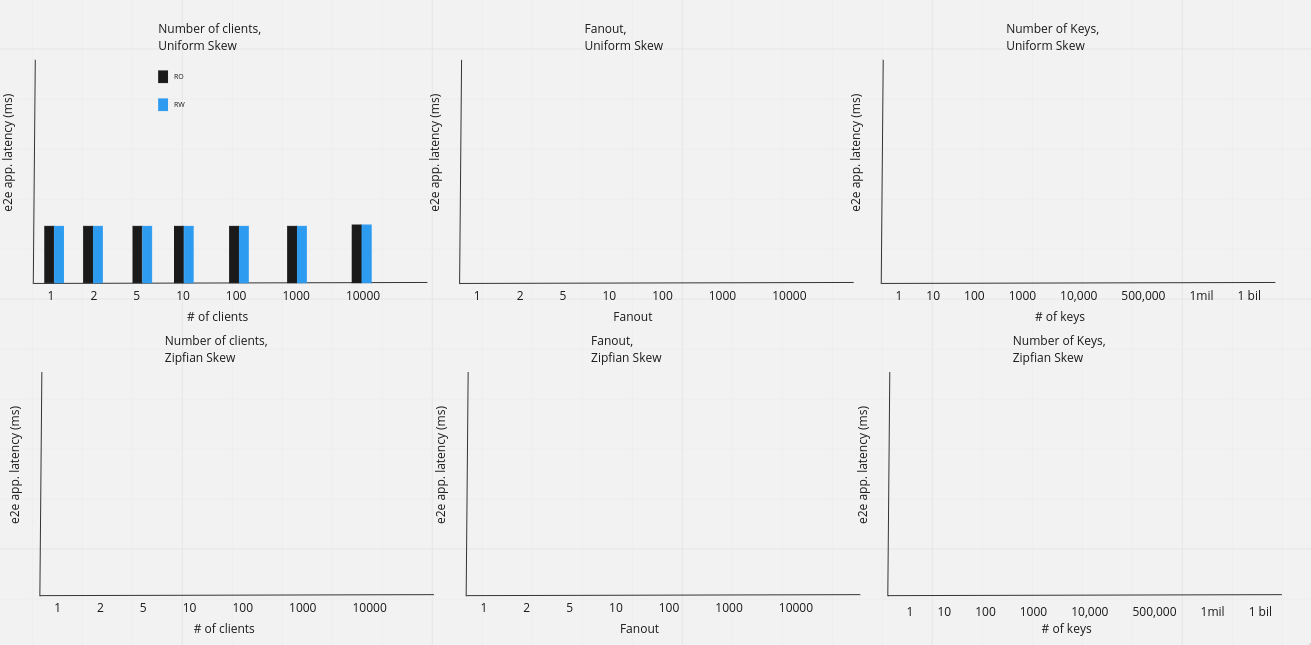
\includegraphics[scale=.36]{microbenchmarks.png}
\caption{Microbenchmarks.}
\label{fig:microben}
\end{figure*}

We are particularly interested in seeing how load (clients+fanout) and contention (key skew) impact the performance of the MDL protocol. 
\begin{enumerate}
    \item With \textbf{increased load}, we expect steady increase in latency at a slow rate, since the protocol should be robust to higher load due to the batching.
    \item With \textbf{increased contention}, we expect uniform slowdown in the face of contention as well since the shards with hot keys will be coordinating requests to other shards at a slower rate
\end{enumerate}  

The contention is most sensitive to
\begin{itemize}
    \item the number of clients \wl{I would vary this for every plot and show throughput/latency graphs}
    \item the fanout \wl{I agree, this is an important parameter to vary}
    \item the skew \wl{I agree, this is an important parameter to vary}
    \item the number of keys \wl{I'd just use ``a lot'' like 1M, 10M}
    \item type of request \wl{I agree, this is an important parameter to vary}
\end{itemize}

We show 6 subplots in figure \ref{fig:microben}, where we vary each of these variables to see the fine grained impact.

We expect to see:
\begin{enumerate}
    \item num of clients: an increase in latency. since the logs will be longer, more to process at each shard
    \item fanout: an increase in latency, same as \# of clients.
    \item skew: an increase in latency, "hot" shards will be slow to coordinate keys at other "cold" shards
    \item num of key: should see decrease in latency, better distribution across shards
    \item type of request: RO will have no coordination, RW will have coordination and thus intershard communication
\end{enumerate}

Some todos:
\begin{itemize}
    \item TODO show plots for system-level throughput
    \item TODO should also probably vary zipfian
\end{itemize}

\subsection{Scaling Number of Shards}
\label{sec:shards}
In this section, we show how the MDL e2e application latency scales with the number of shards. 

As shown in figure \ref{fig:shard-scaling}, we expect app-level request latency will \textbf{scale very well with an increased number of shards.} Assuming we hold the number of clients, fanout, skew/keyspace, and inter-shard RTT values constant, then the protocol shouldn't induce a significantly greater overhead with more shards, and we'd expect to see improved latency for the same load sent to a system configured with fewer shards. 
\begin{enumerate}
    \item In fact, since an increasing number of shards will likely balance the load at each shard, \textbf{the per-shard processing and reordering will be faster, contributing to a speedup} (shorter logs). 
    \item The competing factor that will contribute to an increase in latency is the property that coordination will be across potentially more varied distances. Moreover, with more shards, the \textbf{likelihood of failure increases, also impacting possible coordination slowdowns}.
\end{enumerate}


\begin{figure}[!htb]
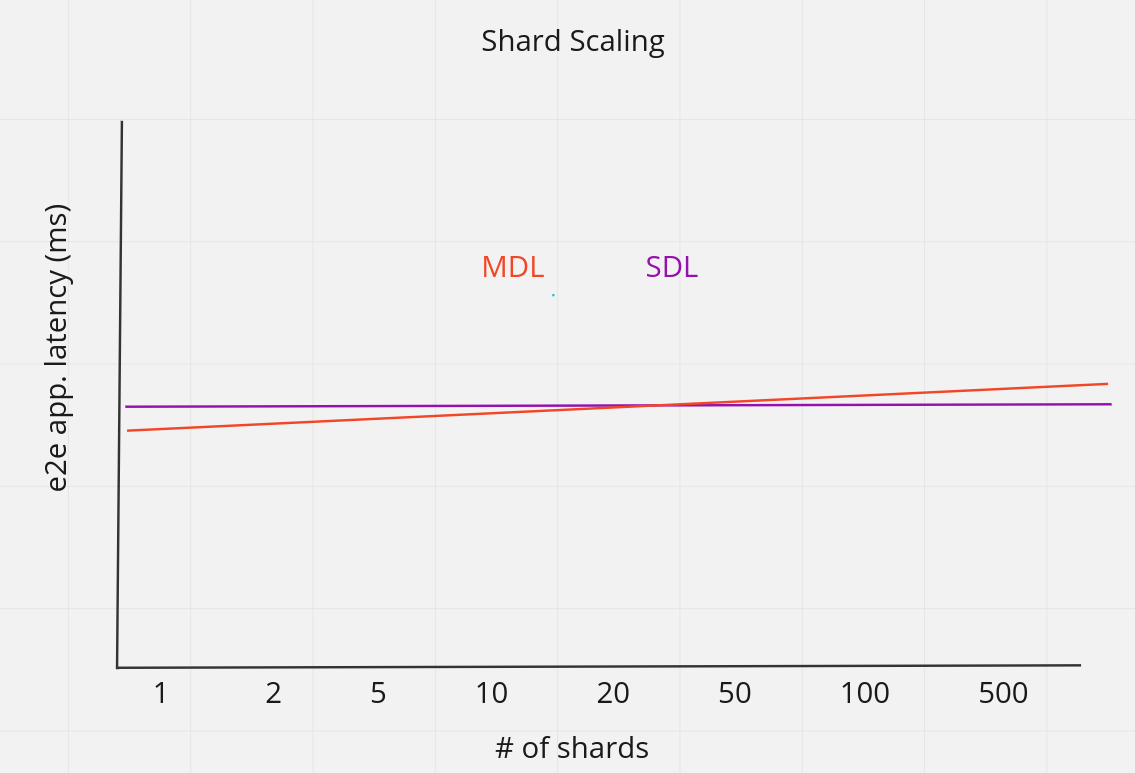
\includegraphics[scale=.20]{shard_scaling.png}
\caption{Multi-sharded MDL with increasing number of shards.}
\label{fig:shard-scaling}
\end{figure}

\subsection{MDL with Geo-rep in the Wide Area}
\label{sec:wide}
We show the e2e app. latency for varying inter-shard latency (which we call the wide area **this might be wrong terminology) and inter-replica latency (which we call geo-replication, also might be wrong terminology).

\begin{figure}[!htb]
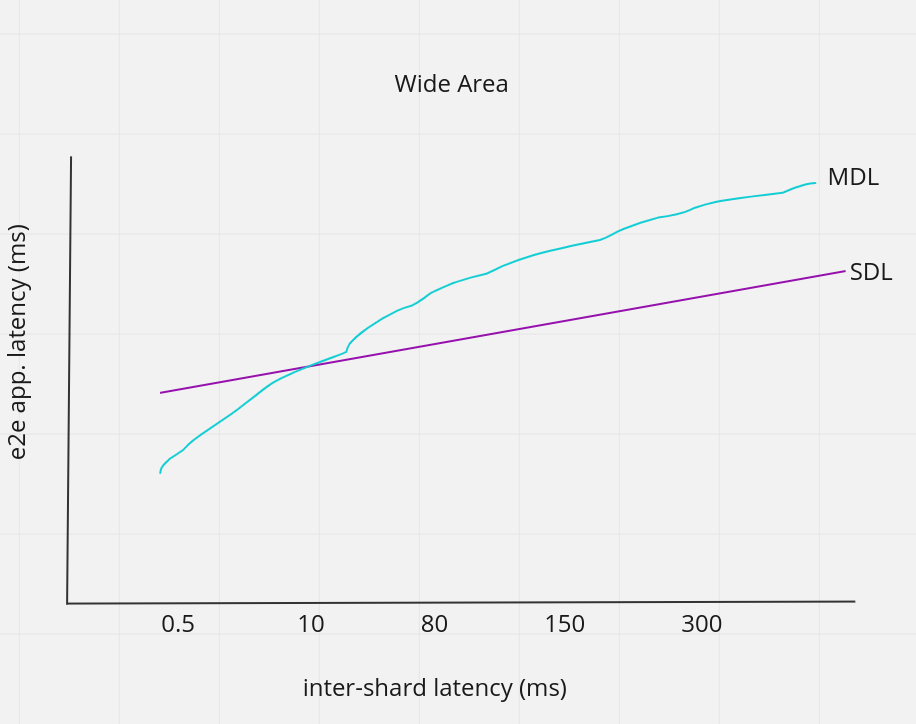
\includegraphics[scale=.24]{wide-area.png}
\caption{Multi-sharded MDL in the Wide Area}
\label{fig:wide-area}
\end{figure}
In figure \ref{fig:wide-area}, if we assume each shard is in a single data center (low inter-rep latency), with increasing inter-shard latency, \textbf{we expect the e2e app. latency for MDL to increase, since the inter-shard communication will take longer} which is fundamentally necessary for the protocol. We expect a small increase for SDL as well, since each subrequest will take a variable length of time, depending on which shard it must visit, but not a significant increase.

In figure \ref{fig:geo-rep}, if we assume a large inter-shard latency, as we increase the inter-replica latency, SDL latency will increase, but \textbf{we expect MDL latency to increase at a slower rate. This is because we can overlap} the inter-replica round trips that have to take place for committing log entries with the inter-shard round trips that have to take place to determine conflicts for log entries.
\begin{figure}[!htb]
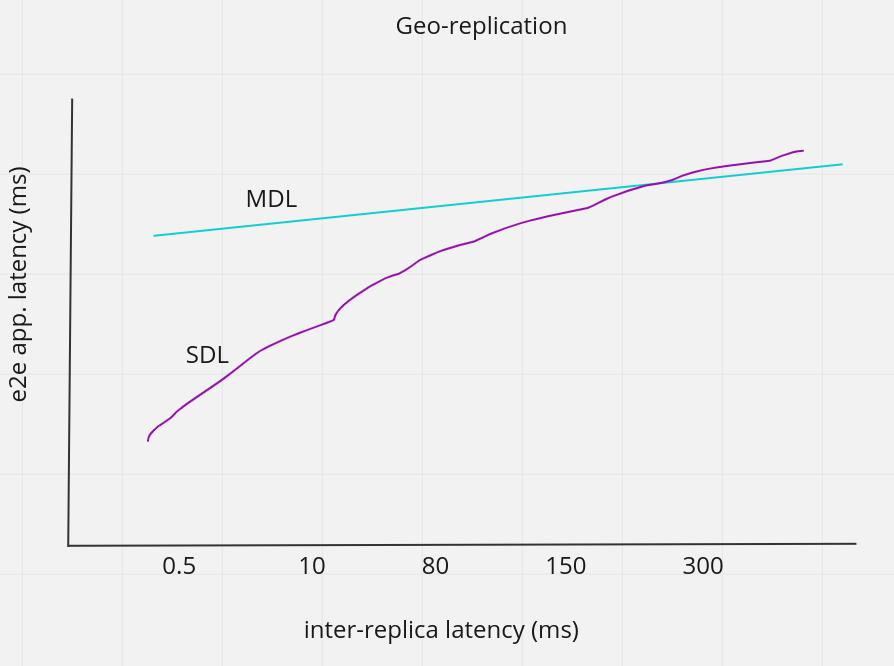
\includegraphics[scale=.25]{geo-rep.png}
\caption{Multi-sharded MDL with Geo-replication.}
\label{fig:geo-rep}
\end{figure}

\subsection{Applications on MDL}
\label{sec:apps}

As described in prior sections, we built a tool to automatically transform applications built to interact with SDL backends to interact with MDL backends, maintaining external equivalence. In this section we select 3 representative applications, A1, A2, A3, and show that when transformed with our tool, all 3 see an improvement in e2e latency. We use DeathStar to benchmark the applications.

A1 is an application that ....

A2 is an application that ...

A3 is an application that ...

We expect transformed applications that have a large degree of data parallelism and are read heavy running on MDL backends to see the largest e2e latency improvements over their pre-transformed counterparts running on SDL backends.

Jeff is still looking for these applications at the moment -- it would be good to pick applications that are read heavy and some that are mixed. All should include varying degrees of data parallelism, to show how some improve after the transformation more than others.